
\lhead[\chaptername~\thechapter]{\rightmark}

\rhead[\leftmark]{}

\lfoot[\thepage]{}

\cfoot{}

\rfoot[]{\thepage}

\chapter{Data}


\section{Data sources}

The data used in this thesis is provided by Ericsson site in Link�ping,
Sweden. Ericsson\footnote{https://www.ericsson.com/}, founded by
Lars Magnus Ericsson in 1876, is one of the world\textquoteright s
leaders in the telecommunication industry. The company provides services,
software products, and infrastructure related to information and communications
technology (ICT). Its head quarter is located in Stockholm, Sweden.
Ericsson continuously expands its services and products beyond telecommunication
industry such as mobile broadband, cloud services, transportation,
and network design.

\begin{figure}[h]
\begin{centering}
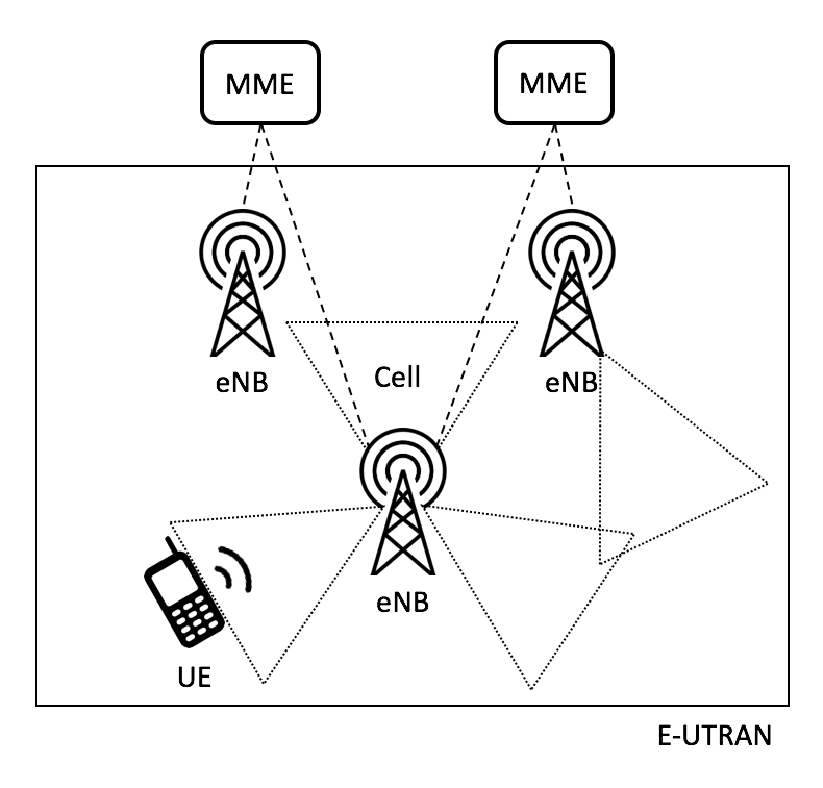
\includegraphics[scale=0.55]{picture/LTE}
\par\end{centering}
\caption{LTE architecture overview}
\label{lte}
\end{figure}

LTE, widely known as 4G, is a radio access technology for wireless
cellular communications. The high-level network architecture of LTE
is shown in \ref{lte} and is described as follows \citep{dahlman20134g}.
The E-UTRAN, an official standard name for the radio access network
of LTE, is the entire radio access network. It handles the radio communication
between the User Equipment (UE) or mobile device and the base stations
called eNB. Each base station controls and manages radio communications
with multiple devices in one or more cells. Several base stations
are connected to a Mobility Management Entity (MME), which is a control-node
for the LTE network. MME establishes a connection and runs a security
application to ensure that the UE is allowed on the network. In LTE
mobile network, multiple UEs are connected to a single base station.
A new UE performs a cell search procedure by searching for an available
eNB when it first connects to the network. Then, the UE sends information
about itself to establish a link between the UE and the eNB. 

Network procedures that will be briefly described here are \emph{Paging}
and \emph{Handover}. Paging is used for the network setup when a UE
is in an idle mode. If a MME wants to notify a UE about incoming connection
requests, the MME will send paging messages to each eNB with cells
belonging to the Tracking Area (TA) where the UE is registered. UE
will wake up if it gets the Paging message and will react by triggering
a Radio Resource Control (RRC) connection request message. Handover
is a process of changing the serving cells or transferring an ongoing
call from one cell to another. For instance, if the UE begins to go
outside the range of the cell and enters the area covered by another
cell, the call will be transferred to the new cell in order to avoid
the call termination. 

Ericsson makes a global \emph{software release} in roughly 6-month
cycles i.e., two major releases per year. Each of these releases contains
a bundle of features and functionalities that is intended for all
the customers. The software release is labeled with \emph{L} followed
by a number related to the year of release and a letter either \emph{A}
or \emph{B,} which generally corresponds to the $1^{st}$ and $2^{nd}$
half of that year. Ericsson opens up a track for each software release
and begins a code integration track. This track becomes the main track
of the work or the focal branch for all code deliveries. There are
hundreds of teams producing code, and each team commits its code to
this track continuously. In order to create a structure for this contribution,
a daily \emph{software package} is built which can be seen as a snapshot
or a marker in the continuous delivery timeline. This software package
is then run through various automated test loops to ensure that there
are no faults in the system. The software packages are named \emph{R,}
and followed by one or more numbers, which is then followed by one
or more letters. \emph{R} stands for Release-state. To summarize,
each software package is a snapshot in the code integration timeline.
\ref{release} presents a relationship between a software release
and software packages. 

\begin{figure}[H]
\begin{centering}
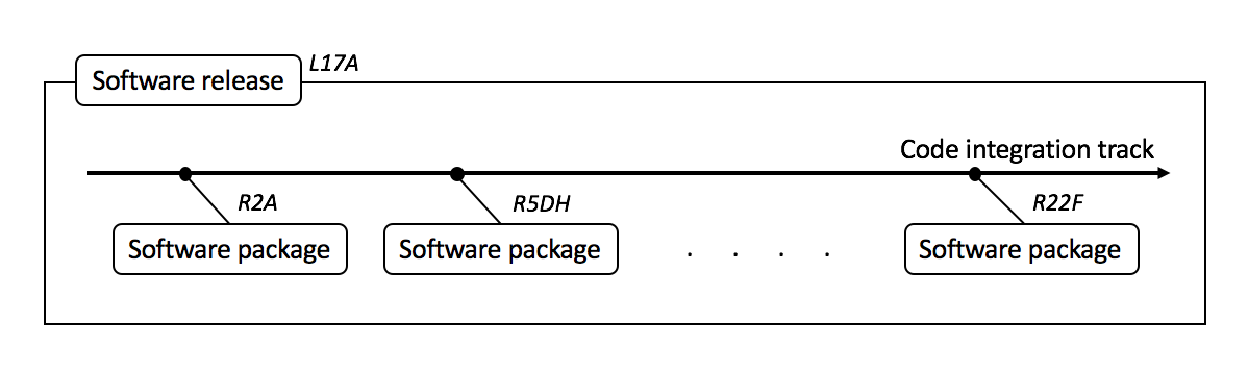
\includegraphics[scale=0.55]{picture/Release}
\par\end{centering}
\caption{An example of one software release that begins a code integration
track. Several software packages are launched in the timeline.}
\label{release}
\end{figure}

There are thousands of automated tests performed. Each test belongs
to a particular suite of tests, which belong to a particular Quality
Assurance (QA) area. For this thesis, only a subset of test cases
belonging to QA Capacity area, that focus on signaling capacity, is
used. The QA Capacity is responsible for testing and tracking test
cases related to eNB capacity. Each one of these test cases has a
well-defined traffic model that it tries to execute. The traffic model,
in this context, means certain intensity (per second) of procedures
which can be seen as stimuli in the eNB. Basically simulating the
signaling load from a large number of UEs served simultaneously by
the eNB. The eNB then increments one or more counters for each one
of these procedures or stimuli that it detects. These counters are
called local events and represented by \emph{EventsPerSec}. 

A logging loop is started during the execution of these test cases
of QA Capacity, signaling capacity. The logging loop collects several
metrics, and a subset of these metrics is what this thesis is currently
studying. Once the logging loop is finished, it is written to a log
file. Then, there are cron jobs that slowly scan through this infrastructure
once a day to find latest logs and do a post-processing. The final
output is either CSV data or JSON encoded charts. The flowchart of
this process is illustrated in \ref{sw}.

\begin{figure}[H]
\begin{centering}
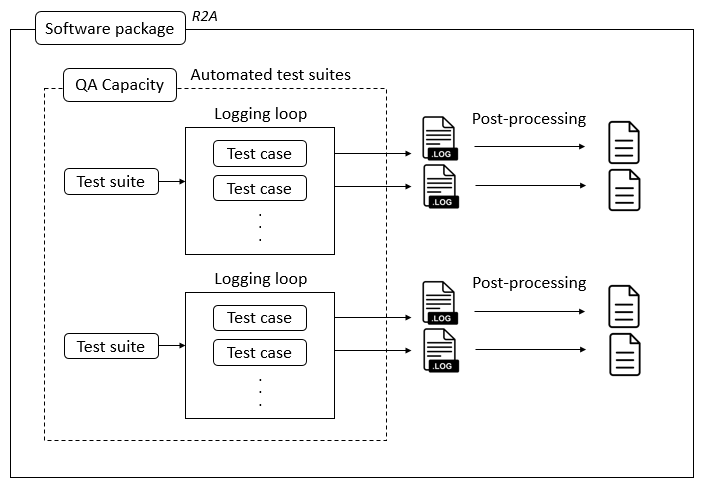
\includegraphics[scale=0.7]{picture/SW}
\par\end{centering}
\caption{An example of one software package. First, QA Capacity automated test
suites is started. For each test suite, a logging loop is started
and a log is produced for each test case. The log file is fed to post-processing
tools, and the data output is obtained.}
\label{sw}
\end{figure}


\section{Data description}

The data used in the thesis contains 2,781 test cases. It is collected
on 20 January 2017 and is extracted from log files produced by test
cases. There are different types of test cases which are being executed
in the automated test suites. Each test case is viewed as an observation
in the data. The following are the variables in the data:

\paragraph{Metadata of test case}
\begin{itemize}
\item Timestamp: Date and time when a test case is being executed (yy-dd-mm
hh:mm:ss) 
\item NodeName: IP address or the name of a base station
\item DuProdName: Product hardware name
\item Fdd/Tdd: Different standard of LTE 4G Technology. FDD and TDD stand
for Frequency Division Duplex and Time Division Duplex, respectively.
\item NumCells: Number of cells in the base station
\item Release: Software release 
\item SW: Software package
\item LogFilePath: Path for log file produced by a test case
\end{itemize}

\paragraph{CPU}
\begin{itemize}
\item TotCpu\%
\item PerCpu\%
\item PerThread\%
\item EventsPerSec 

The EventsPerSec variable, or Event intensity, contains several local
events that can be used when defining the test cases. Apparently,
there is no fixed number of local events in this variable as different
test cases involve different testing procedures. The local events
along with their values are also varied depending on which types of
test cases are being executed. An example of the local events in test
cases is shown in \ref{eventspersec}.

\begin{table}[H]
\caption{List of local events in the test cases separated by a tab character}
\label{eventspersec}
\centering{}%
\begin{tabular}{|c|>{\centering}p{11cm}|}
\hline 
Test case & EventsPerSec\tabularnewline
\hline 
\hline 
1 & ErabDrbRelease=166.11 ErabSetupInfo=166.19 PerBbUeEventTa=167.98 PerBbUetrCellEvent=12.00
ProcInitialCtxtSetup=166.20 RrcConnSetupAttempt=166.21 RrcConnectionRelease=166.11
S1InitialUeMessage=166.20 UplinkNasTransport=32.06

...\tabularnewline
\hline 
2 & ErabDrbAllocated=641.30 EventS1InitialUeMessage=142.20 McRrcConnectionRequest=142.99
McX2HandoverRequest=98.70 Paging=1399.94 PerBbLcgEvent=26.14

...\tabularnewline
\hline 
... & ...\tabularnewline
\hline 
\end{tabular}
\end{table}

\end{itemize}

\section{Data preprocessing}

The relevant aspects of the data preprocessing step are describe here.
The dataset, which spans three software releases, is split into three
datasets according to the software release. In this thesis framework,
Ericsson software releases will be referred as software release A,
B, and C. 

The test cases in each dataset are sorted by their software package
version, which is named alphabetically. The name of the software package
is used as a time point in the time series.

Some test cases are filtered out in the preprocessing step because
the test cases are not always executed properly. The problem is either
no traffic is generated during the test case or the data is not logged.
This usually results in a missing value in the \emph{EventsPerSec}
field, which causes the test case to be incomplete. The local events
in the \emph{EventsPerSec} field are used to define the test case
type and will also be used as predictor variables for a further analysis.
If there is no value or no local events in this field, the particular
test case and all the data related to the test case is ignored. These
incomplete test cases in the data are accounted for four percent of
all the test cases in the data.

In \ref{eventspersec}, it can be seen that the \emph{EventsPerSec}
stores multiple values separated by a tab character. These tab-separated
values in the field are split into columns. A function is implemented
to perform this process and is further described in details in \ref{sec:EventsPerSec}.
The process is done in order to turn its local events and values,
which characterize the test case, into usable parameters. These parameters
are later on used as predictor variables when the Markov switching
model is applied.

Each software release consists of several software packages. For each
specific software package, numerous test cases are executed. Since
a software package acts as a time point in the time series, the result
is rather difficult to visualize using every executed test case for
each software package. Hence, the test case that has the lowest value
of the CPU utilization (or minimum value of \emph{TotCpu\%}) is selected
to represent a performance of the specific software package. Although
taking an average of multiple runs for test cases in the software
package appears to be a good approach, it does not yield the best
outcome in this case. The first reason is that manipulating data can
easily be misleading. Another important reason for not using the average
value of the CPU utilization is that the essential information in
the test case could be lost. Each test case has its own local events
in \emph{EventsPerSec} field that is used for identifying the test
case. The details of these local events will be absent if the CPU
utilization of the test case is averaged. It is, therefore, settled
to keep the original data and always use the unmanipulated data to
visualize the time series.

After performing all the steps described above, the datasets of the
software release A, B, and C consist of 64, 241, and 144 test cases,
respectively. Lastly, each dataset with particular software release
is divided into two subsets. Ninety percents of the dataset is used
for training the model and the remaining ten percents is left out
for testing the model. 

In total, there are one response variable and six predictor variables.
\ref{data} shows the name of the variables and their descriptions.
These predictor variables have been analyzed and are chosen by an
area expert. The first three predictor variables are local events
of the test case, which can be found in the \emph{EventsPerSec. }They
are considered to be the main components in defining the test case
type. The last three variables are considered as the test environment.
These variables appear to have a high influence to the CPU utilization.

\begin{table}[H]
\caption{List of the selected variables followed by its type and unit measure }
\label{data}
\centering{}%
\begin{tabular}{|l||l|l|l|}
\hline 
Variable & Name & Type & Unit\tabularnewline
\hline 
\hline 
Response  & TotCpu\% & Continuous & Percentage\tabularnewline
\hline 
Predictor  & RrcConnectionSetupComplete & Continuous & Per second\tabularnewline
 & Paging & Continuous & Per second\tabularnewline
 & X2HandoverRequest & Continuous & Per second\tabularnewline
 & DuProdName & Categorical & \tabularnewline
 & Fdd/Tdd & Binary & \tabularnewline
 & NumCells & Categorical & \tabularnewline
\hline 
\end{tabular}
\end{table}


